\section{Comparative Analysis}

The Indian Buffet Process (IBP) is compared with the Chinese Restaurant Process~\cite{crp2004hierarchical}, which is also a Bayesian nonparametric method to discover latent features in a given dataset. My implementation with simulated data is also compared with a Matlab version~\cite{ibp2012code} and a Python version~\cite{ibpgithub} online.

\subsection{Indian Buffet Process (IBP) vs Chinese Restaurant Process (CRP)}

As mentioned in Section~\ref{sec:intro}, the Chinese Restaurant Process (CRP)~\cite{crp2004hierarchical} is an algorithm of customers' seating in a Chinese restaurant with infinite capacity. The first customer sits at an empty table with probability 1. Then starting from time 2, a new customer chooses randomly at either to the left of one of the previous customers, or at a new, unoccupied table.\\

Both IBP and CRP model latent factors and perform dimensionality reduction (reduce the images or objects to latent features). They also both allow an infinite array of objects. Nevertheless, they solve different problems: IBP allows each customer to be assigned to multiple components (dishes), while CRP assigns each customer to a single component. Figure~\ref{fig:CRP} from Gershman's and Blei's paper~\cite{gershman2012tutorial} illustrates the difference between draws of IBP and CRP.

\begin{figure}[!ht]
\centering
    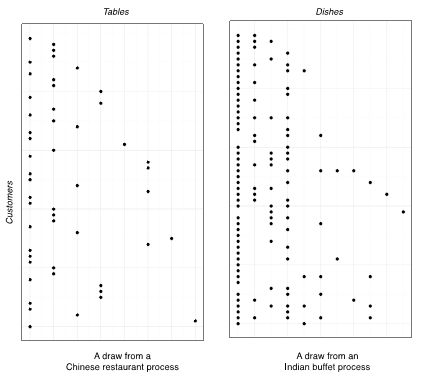
\includegraphics[width=0.65\linewidth]{IBP_vs_CRP.png}
    %\vspace{-20pt}
    \caption{Indian Buffet Process (IBP) vs Chinese Restaurant Process (CRP)~\cite{gershman2012tutorial}}
    \label{fig:CRP}
\end{figure}

\subsection{Indian Buffet Process: Another Matlab Version Online}
% Matlab code: Five times faster than my Python version
% Show their results
% Figure: Profiling table

The Matlab version I compared with is Yildirim's IBP sample code~\cite{ibp2012code}, and the simulated dataset in both versions of code are the same as in Section~\ref{sub:simulated}. For 1000 iterations of Gibbs sampling, the Matlab code takes about 400 seconds to run, while my Python version takes approximately 2000 seconds. The Matlab code is not only five times faster than my Python code, but also gives the correct four latent features, as in Figure~\ref{fig:matlabresults}.\\

The truncated profiling results using the Matlab tool "Run and Time" for the functions \texttt{sampler, likelihood, calInverse} are listed in Figure~\ref{fig:ibp2012matlab}. The column "Self time" indicates the time spent in a function, but it includes the overhead time of profiling and excludes the time spent in its child functions. The function \texttt{sampler} refers to the whole Gibbs sampler; \texttt{likelihood} is the likelihood calculation, and \texttt{calInverse} is the implementation from Griffiths' and Ghahramani's paper\cite{griffiths2005detailed}, to compute $\mathbf{M}$ faster when only one $\mathbf{z_i}$ is changed. 

\begin{figure}[!ht]
\centering
    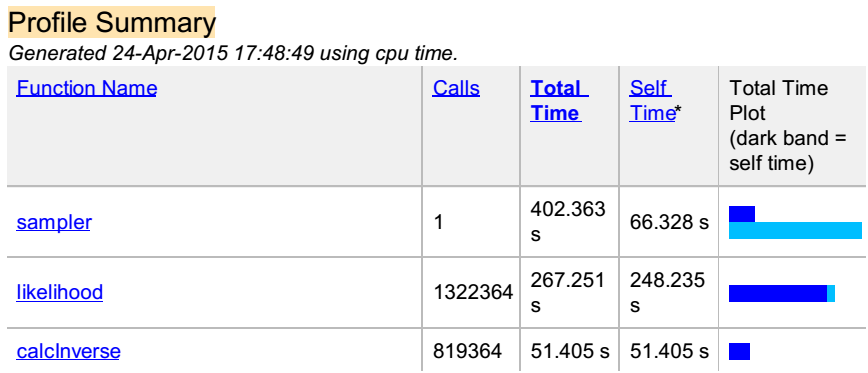
\includegraphics[width=0.8\linewidth]{IBP_MATLABcode/matlab_code_profiling_summary.png}
    %\vspace{-20pt}
    \caption{Matlab code: Profiling results (truncated)}
    \label{fig:ibp2012matlab}
\end{figure}

\begin{figure}[!ht]
\centering
    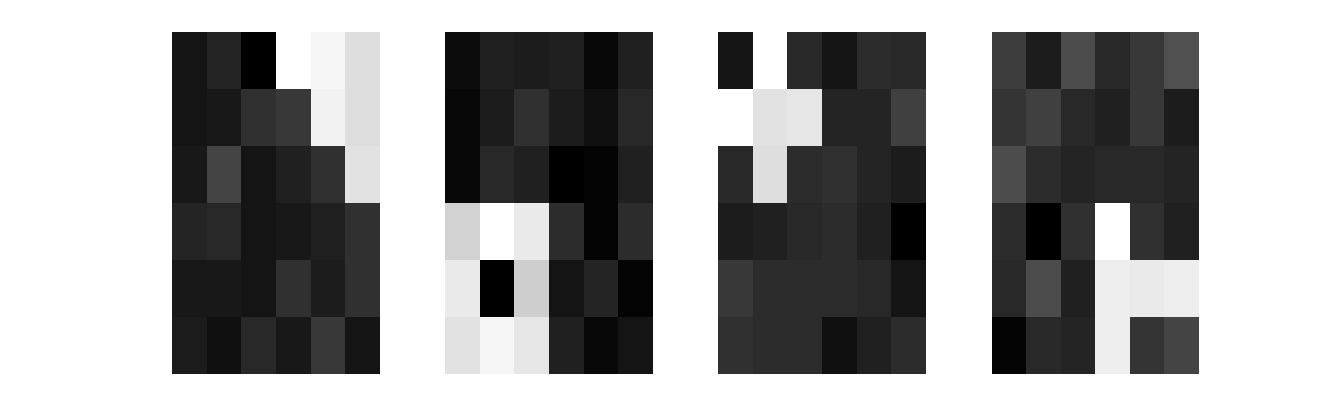
\includegraphics[width=0.8\linewidth]{IBP_MATLABcode/Fig4_results.png}
    %\vspace{-20pt}
    \caption{Matlab code: Latent features discovered}
    \label{fig:matlabresults}
\end{figure}

\subsection{Indian Buffet Process: Another Python Version Online}

The other Python version I compared with is Andrzejewski's PyIBP~\cite{ibpgithub} on GitHub. This version has two advantages -- speed and organization, but the two drawbacks are result inconsistency and difficulty in execution (lack of Makefile). Note that these two disadvantages of PyIBP can be removed by adding small lines of code.\\

% Accelerated Gibbs Sampling
First, the accelerated Gibbs sampling~\cite{andrzejewski2011accelerated,doshi2009accelerated} makes the code much faster, and only five iterations are needed to generate the results. The accelerated Gibbs sampling not only exploits the conjugate normal prior and likelihood by rank-one $\mathbf{M}$ updates, but also uses slice sampling~\cite{andrzejewski2011accelerated} to decompose sampling from the unnormalized posterior distribution of $\mathbf{X}$ into discrete steps of uniform distributions. For example, sampling from an arbitrary unnormalized distribution $\widetilde{p}(y)$ can be performed by the following steps, given a current value $y$ and window boundaries $(L,R)$ where $y$ lies within:

\begin{enumerate}
\item Sample $u \sim \text{Unif}(0,\widetilde{p}(y))$
\item Sample $\widehat{y} \sim \text{Unif}(L,R)$
\item Accept new $\widehat{y}$ value if $\widetilde{p}(y) > u$, else reject
\end{enumerate}

In this way, the expensive matrix multiplication in the normal likelihood kernel can be avoided. \\

Second, the PyIBP code is organized; the author generated the modules \texttt{PyIBP.py} and \texttt{scaledimages.py}, and the user can run the example file without needing to learn much about the IBP process.\\

However, the two drawbacks can cause problems in implementation, but these problems are easy to solve. To begin with, sometimes the PyIBP code produces excellent results like Figure~\ref{fig:PyIBPbest}, but sometimes the discovered latent features are noisy, such as in Figure~\ref{fig:PyIBPworst}. In both figures, the top four images are the ground-truth features, and the bottom shows the generated results. Setting a fixed random seed can ensure the results to be reproducible. For another disadvantage, a Makefile does not exist in the original PyIBP code, so it takes some time for users to figure out how to execute the PyIBP example. Therefore, I wrote a Makefile for convenience of execution.

\begin{figure}[!ht]
\centering
    \begin{minipage}{0.5\linewidth}
    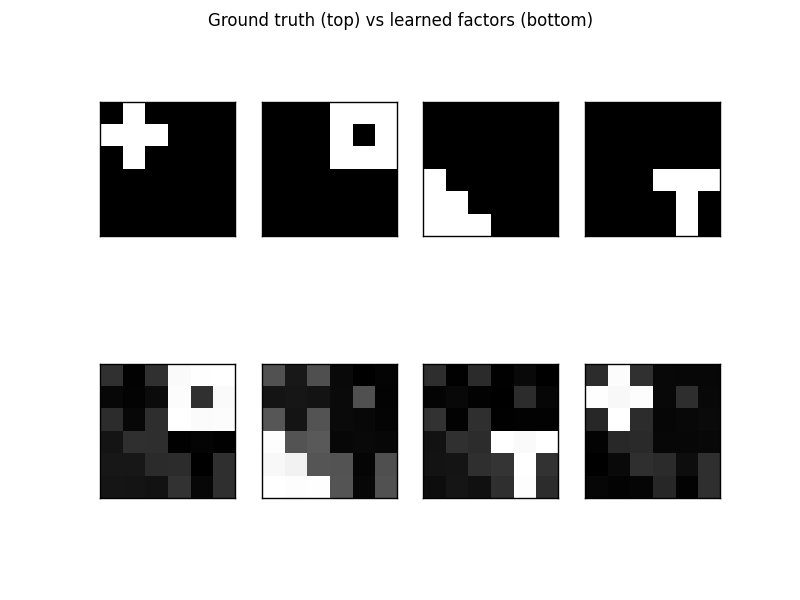
\includegraphics[width=\linewidth]{PyIBP/example/PyIBP_comparison_best.png}
    %\vspace{-20pt}
    \captionof{figure}{PyIBP code: Best results}
    \label{fig:PyIBPbest}
    \end{minipage}%
    \begin{minipage}{0.5\linewidth}
    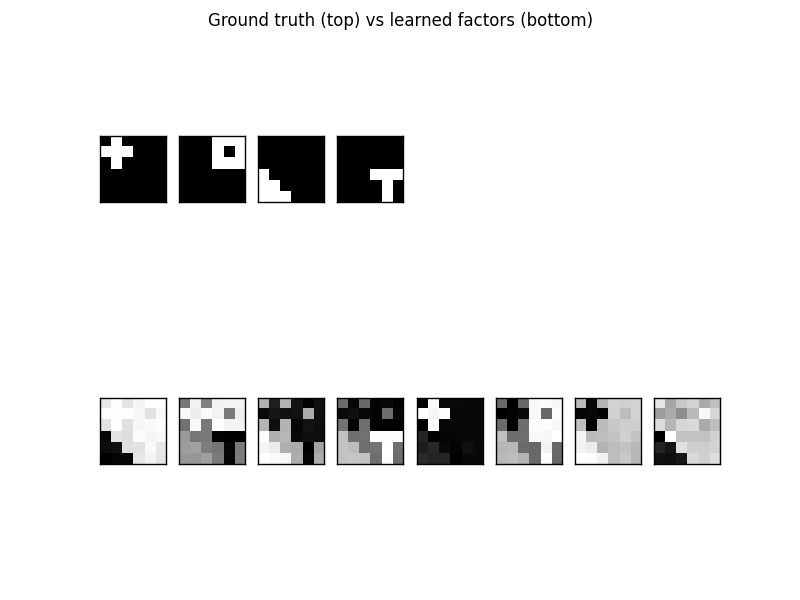
\includegraphics[width=\linewidth]{PyIBP/example/PyIBP_comparison_worst.png}
    %\vspace{-20pt}
    \captionof{figure}{PyIBP code: Worst results}
    \label{fig:PyIBPworst}
    \end{minipage}
\end{figure}

%### PyIBP (GitHub repository)
%- Advantage 1: Really fast, only 5 samples required
%- Advantage 2: Organized -- the author generates the modules PyIBP.py and scaledimages.py
%- Hence the user does not need to learn much about the IBP process
%- -----------------------------------------
%- Drawback 1: Inconsistency -- sometimes gets good results, sometimes really bad
%- Randomized parts: initV, sampleX, sampleZ by a normal distribution
%- Show both figures for comparison -- ground truth factor-feature weights (top) + learned factor-feature weights (bottom)
%- My code sets a random seed to ensure reproducibility of results.
%- Drawback 2: No Makefile exists, so I wrote one for it.
%-  def initV(self):
%        """ Init latent feature weights V accoring to N(0,1) """        
%        for (i,k) in zip(*self.ZV.nonzero()):
%            self.ZV[i,k] = NR.normal(0,1)
